\chapter{Two Degrees of Freedom (2-DOF) Controller} 
In this chapter, we discuss the implementation of a 2-DOF controller using the SBHS. We also cover the basics of 2-DOF 
controller theory and design. 
%\begin{figure}
%\centering
%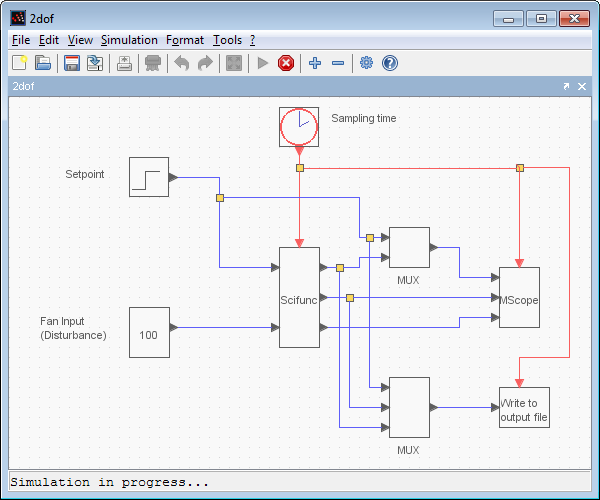
\includegraphics[width=0.9\linewidth]{2-DOF_manual/2dof_xcos.png}
%\caption{Xcos interface for this experiment}
%\label{Xcos_2dof}
%\end{figure}
%We have used Scilab with Xcos as an interface for sending and receiving data. This interface is shown in Fig.\ref{Xcos_2dof}. Fan speed and Heater current are the two inputs to the system. For this experiment, the heater current is used as a control effort generated by inputting the various 2-DOF controller parameters like Rc, Sc, Tc and gamma. The fan input could be thought of as an external disturbance.
\section{Introduction to 2-DOF Controller}
Controllers are broadly divided into two categories: feedback and feed forward controllers. Feed forward controllers 
are those that take control action before a disturbance affects the plant. But this requires an ability to sense the
disturbance accurately. Moreover, exact knowledge of the plant is also needed. As a result, a feed forward control 
strategy is rarely used alone. 

A feedback control strategy is shown in figure \ref{fb}. The reference $r$ and the output $y$ are continuously compared 
to generate error $e$, which is fed to the controller $G_c(z)$, to take appropriate control action. $u$ is the controller 
output that is fed to the plant. Unlike feed forward controllers, exact knowledge of the plant $G(z)$ and the disturbance
$v$ is not necessary in this case. Feedback controllers are further classified as One Degree of Freedom (1-DOF) controllers
and Two Degrees of Freedom (2-DOF) controllers.  Degree of freedom refers to the number of parameters that are free to vary
in a system. A higher degree of freedom controller makes the plant less susceptible to disturbances.
\begin{figure}
\begin{center}
\begin{tikzpicture}[auto, node distance=2cm]
\node[input, name=input]{};
\node[sum,right of=input](sum){};
\draw[->](input) -- node{$r$}(sum);
\node[block, right of=sum](gc){$G_c(z)$};
\draw[->](sum)--node{$e$}(gc);
\node[block, right of=gc, node distance=3cm](g){$G(z)$};
\draw[->](gc)--node{$u$}(g);
\node[sum, right of=g,pin={[pinstyle] above:$v$},node distance=2cm](sum2){};
\draw[->](g)--node{}(sum2);
\node[output,right of=sum2,node distance=1cm](output){};
\draw[->](sum2)--node[name=y]{$y$}(output);
\draw [->] (y)--(8.58,-1.5)-|(sum)node[pos=0.88] {$-$};
\end{tikzpicture}
\end{center}
\caption{Feed back control strategy}
\label{fb}
\end{figure}


\begin{align}
\intertext{The expression for output, $Y(z)$ of the system shown in figure \ref{fb} is given by}
Y(z)&=\frac{G(z)G_c(z)}{1+G(z)G_c(z)}R(z)+\frac 1{1+G(z)G_c(z)}V(z)
\intertext{This expression can be written in mixed notation \cite{kmmdc09} as}
y(n)&=\frac{G(z)G_c(z)}{1+G(z)G_c(z)}r(n)+\frac 1{1+G(z)G_c(z)}v(n)
\intertext{Let,}
T(z)&=\frac{G(z)G_c(z)}{1+G(z)G_c(z)} , \,
S(z)=\frac 1{1+G(z)G_c(z)}
\intertext{Therefore,}
y(n)&=T(z)r(n)+S(z)v(n)
\end{align}
The controller has to track the reference input as well as eliminate the effect of external disturbance. So ideally, we want
T = 1 and S = 0. But, it is not possible to achieve both the requirements simultaneously using this control strategy. This 
control strategy is called {\tt One Degree of Freedom}, abbreviated as 1-DOF.

A {\tt Two Degrees of Freedom} controller is as shown in figure \ref{2dof}. Here, $G_b$ and $G_f$ together 
constitute the controller. $G_b$ is in the feedback path and is used to eliminate the effect of disturbances,
whereas $G_f$ is in the feed forward path and is used to help the output track the reference input. 
\begin{figure}
\begin{center}
\begin{tikzpicture}[auto,node distance=2cm]
\node[input,name=input](input){};
\node[block,right of=input](gf){$G_f$};
\draw[->](input) -- node{$r$}(gf);
\node[sum,right of=gf,node distance=2cm](sum1){};
\draw[->](gf)--node{}(sum1);
\node[block,right of=sum1](g){$G$};
\draw[->](sum1)--node{$u$}(g);
\node[sum,right of=g,node distance=2cm](sum2){};
\draw[->](g)--node{}(sum2);
\node[output, right of=sum2,node distance=1cm](output){};
\draw[->](sum2)--node[name=y]{$y$}(output){};
\node[block, above of=sum2](h){$H$};
\draw[->](h)--node{$v$}(sum2);
\draw[->](8.015,3.8)--node{$d$}(h);
\node[block, below of=g](gb){$G_b$};
\draw[->](y)|-(gb);
\draw[->](gb)-|node[pos=0.99]{$-$}(sum1);
\end{tikzpicture}
\end{center}
\caption{2DOF Feed back control strategy}
\label{2dof}
\end{figure}


The expression for control effort $u$ in figure \ref{2dof} is given by
\begin{align}
u(n) & = r(n)G_f - y(n)G_b
\intertext{Let}
G_b &= \frac{S_c}{R_c} , G_f = \frac{T_c}{R_c}
\intertext{where $R_c$, $S_c$ and $T_c$ are polynomials in $z^{-1}$.}
\intertext{We get}
R_c(z)u(n)&=T_c(z)r(n)-S_c(z)y(n)\label{desired}
\intertext{Consider a plant whose model is given by}
A(z)y(n)&=z^{-k}B(z)u(n)+v(n)\label{model}
\intertext{Substituting equation \ref{desired} in equation \ref{model}, we get}
Ay(n)&=z^{-k}\frac{B}{R_c}\bigg[T_cr(n)-S_cy(n)\bigg]+v(n)
\intertext{Solving for $y(n)$,}
\bigg(\frac{R_cA+z^{-k}BS_c}{R_c}\bigg)y(n)&=z^{-k}\frac{BT_c}{R_c}r(n)+v(n)
\intertext{This can also be written as}
y(n)&=z^{-k}\frac{BT_c}{\phi _{cl}}r(n)+\frac{R_c}{\phi _{cl}}v(n)
\intertext{where $\phi_{cl}$ is the closed loop characteristic polynomial given by }
\phi _{cl}&=R_c(z)A(z)+z^{-k}B(z)S_c(z)
\end{align}

We want the following conditions to be satisfied while designing a controller.
\begin{enumerate}
\item The zeros of $\phi _{cl}$ should be inside the unit circle, so that the closed-loop system becomes stable
\item The value of $z^{-k}\dfrac{BT_c}{\phi _{cl}}$ must be close to unity, so that reference tracking is achieved 
\item The value of $\dfrac{R_c}{\phi _{cl}}$ must be as small as possible to achieve disturbance rejection
\end{enumerate}
We shall now see the pole placement controller approach to design a 2-DOF controller.

\section{2-DOF Controller Design using the Pole Placement Method \cite{kmmdc09}}
A 2-DOF pole placement controller is shown in figure \ref{2dofppc}. We will not consider the effect of external
disturbance in the design. The controller will be designed for setpoint tracking. 
\begin{figure}
\begin{center}
\begin{tikzpicture}[auto,node distance=2cm]
\node[input](input){};
\node[block,right of=input](tcbyrc){$\gamma \dfrac{T_c(z)}{R_c(z)}$};
\draw[->](input)--node{$r$}(tcbyrc);
\node[sum,right of=tcbyrc,node distance=2cm](sum1){};
\draw[->](tcbyrc)--node{}(sum1);
\node[block,right of=sum1](plant){$G=z^{-k}\dfrac{B(z)}{A(z)}$};
\draw[->](sum1)--node{$u$}(plant);
\node[output,right of=plant](output){};
\draw[->](plant)--node[name=y]{$y$}(output);
\node[block,below of=plant](scbyrc){$\dfrac{S_c(z)}{R_c(z)}$};
\draw[->](y)|-node{}(scbyrc);
\draw[->](scbyrc)-|node[pos=0.99]{$-$}(sum1);
\end{tikzpicture}
\end{center}
\caption{2-DOF pole placement controller}
\label{2dofppc}
\end{figure}

We want the desired output, $Y_m$, of the system to be related to the setpoint $R$ in the following manner:
\begin{align}
Y_m(z)&=\gamma z^{-k}\frac{B_r}{\phi_{cl}}R(z)\label{modeloutput}
\intertext{$\phi_{cl}$ is the desired closed loop characteristic polynomial obtained from the desired region analysis. 
Please refer to \cite{kmmdc09} for more information on desired region analysis. $\gamma$ is  chosen such that $Y_m$ equals 
the setpoint at steady-state. Therefore $\gamma$ is given by,}
\gamma&=\dfrac{\phi_{cl}(1)}{B_r(1)}
\intertext{Simplifying the block diagram shown in figure \ref{2dofppc} yields}
Y&=\gamma z^{-k}\frac{BT_c}{AR_c+z^{-k}BS_c}R\label{blkdigoutput}
\intertext{We have dropped the argument of $z$ for convenience}
\intertext{We want the output $Y$ of the system to be equal to the desired output $Y_m$.  Equating equations \ref{modeloutput}
and \ref{blkdigoutput} we get}
\frac{BT_c}{AR_c+z^{-k}BS_c}&=\frac{B_r}{\phi_{cl}}\label{comparison}
\intertext{We can expect some cancelations between the numerator and the denominator polynomials in the LHS, thereby making
$deg B_r < deg B$. But the cancelations, if any, must be between $stable$ poles and zeros. One should avoid the cancelation 
of an unstable pole with an unstable zero.}
\intertext{Let us split the factors of the numerator and denominator polynomials, $B$ and $A$, of the plant into $good$ and
$bad$ factors. Therefore, we write $A$ and $B$ as }
A&=A^gA^b, B=B^gB^b
\intertext{We also define $R_c,S_c$ and $T_c$ as}
R_c&=B^gR_1\\
S_c&=A^gS_1\\
T_c&=A^gT_1
\intertext{Hence, equation \ref{comparison} becomes}
\frac{B^gB^bA^gT_1}{A^gA^bB^gR_1+z^{-k}B^gB^bA^gS_1}&=\frac{B_r}{\phi_{cl}}
\intertext{After cancelling out the common factors, we obtain}
\frac{B^bT_1}{A^bR_1+z^{-k}B^bS_1}&=\frac{B_r}{\phi_{cl}}\label{aftercancelation}
\intertext{We obtain,}
B^bT_1&=B_r\label{Br}\\
A^bR_1+z^{-k}B^bS_1&=\phi_{cl}\label{aryabhatta}
\intertext{Equation \ref{aryabhatta} is known as the Aryabhatta's identity and can be used to solve for $R_1$ and $S_1$. 
One can choose $T_1$ in many ways. If we choose $T_1 = S_1$ the 2-DOF controller is reduced to a 1-DOF controller. Let us 
choose $T_1=1$. Therefore equation \ref{Br} becomes }
B^b&=B_r
\intertext{The expression for $\gamma$ now becomes}
\gamma&=\frac{\phi_{cl(1)}}{B^b(1)}
\intertext{and the desired closed loop transfer function will be}
\frac{Y_m(z)}{R(z)}&=\gamma z^{-k}\frac{B^b}{\phi_{cl}}
\end{align}
One can see that the open loop plant model imposes two limitations on the closed loop transfer function.
\begin{enumerate}
\item The bad portion of the open loop model cannot be canceled out and it appears in the closed loop model. 
\item The open loop plant delay cannot be removed or minimized, i.e., the closed loop model cannot be made faster than the 
open loop model.  
\end{enumerate}
\section{2-DOF Pole Placement Controller Design and Implementation using SBHS}
We obtain a first order transfer function of the plant using the step test approach. Refer to the chapter on Step Test 
using SBHS for more details. The model obtained is
\begin{align}
G(s)&=\frac{0.42}{35.61s+1}
\intertext{with a time constant of $\tau = 35.6 s$ and gain $K=0.42$}
\intertext{After discretization with sampling time = 1 s, we obtain}
G(z)&=\frac{0.0116304z^{-1}}{1-0.9723086z^{-1}}
\end{align}
Refer to the Scilab code {\tt myc2d.sci} \footnote{Go the folder {\tt dc} inside the {\tt 2dof\_controller} folder. 
Now go to
the folder {\tt scilab} and locate {\tt myc2d.sci}}.
We shall now define good and bad factors as 
\begin{align*}
A^g&=1-0.9723086z^{-1}\\
A^b&=1\\
B^{g}&=0.0116304\\
B^{b}&=1
\intertext{Let us now define the transient specifications. We choose Rise Time =100 s and Overshoot ($\epsilon$)= 5\%. Number
of samples in one rise time ($N_r$), \cite{kmmdc09}, is calculated as}
N_r&\le\frac{\text{Rise time}}{\text{Sampling time}}\\
&=100\\
\therefore, \omega&=\frac{\pi}{2N_r}\\
&=0.015708\\
\intertext{and}
\rho&\le \epsilon ^{\omega / \pi}\\
&=0.98513
\intertext{The closed loop characteristic polynomial is given by,}
\phi _{cl}&= 1-2\rho cos\omega z^{-1} + \rho ^2z^{-2}\\
&=1-1.9700229z^{-1}+0.9704870z^{-2}
\intertext{Refer to the Scilab code {\tt desired.sci} to calculate $N_r$, $\omega$, $\rho$ and $\phi_{cl}$. The code is 
available in the same location as {\tt myc2d.sci}.}
\intertext{But according to equation \ref{aryabhatta},}
A^bR_1+z^{-k}B^bS_1&=\phi_{cl}
\intertext{Recall that we have not considered external disturbance in the block diagram shown in figure \ref{2dofppc}. 
However, we can still up to some extent take care of the disturbances. This is achieved by using the Internal Model 
Principle. If a model of step is present inside the loop, step disturbances can be rejected \cite{kmmdc09}. We can apply
this by forcing $R_c$ to have this term. A step model is given by}
1(z)&=\frac{1}{1-z^{-1}} = \frac 1{\Delta}
\intertext{Therefore,}
R_c&=B^g\Delta R_1
\intertext{$\Delta$ has a root which lies on the unit circle. Hence it has to be treated as a bad part and should not be canceled out. Hence, we should make sure that all of the occurrences of $R_1$ have this term.}
\end{align*}
Therefore,
\begin{align}
\phi_{cl}&=A^b\Delta R_1+z^{-k}B^bS_1 \label{eqn-new}
\intertext{Hence,}
A^b\Delta R_1+z^{-k}B^bS_1&=1-1.9700229z^{-1}+0.9704870z^{-2} \label{arya-new}
\end{align}
is expression is known as the Aryabhatta Identity and is solved using rigorous matrix calculations. The explanation of 
this operation is not considered here. Refer to \cite{kmmdc09} for more details on Aryabhatta's Identity. Refer to the 
Scilab code {\tt pp\_im.sci}, which is used to split the denominator and numerator polynomials of the plant transfer 
function into good and bad factors, and solving the Aryabhatta's Identity given in equation \ref{arya-new}. On solving 
equation \ref{arya-new}, we get
\begin{align*}
R_c&=0.0116304-0.0229175z^{-1}+0.0112871z^{-2}\\
S_c&=0.0004641-0.0004512z^{-1}\\
T_c&=1-0.9723z^{-1}\\
\gamma&=0.0004641
\end{align*}

All the above calculations are incorporated into a single Scilab code named {\ttfamily twodof\_para.sce} 
\footnote{All the Scilab codes are given at the end of this chapter in the section \ref{2dof-local}}.
\subsection{Procedure to calculate 2DOF parameters using scilab }\label{sec-steps}
The procedure explained here is applicable to both virtual as well as local experiments. The following steps must be executed properly to calculate the controller parameters. 
\begin{enumerate}
\item Change the directory to {\tt 2dof\_controller}. 
\item Execute the command {\tt getd dc/scilab} in the scilab console.
\item Open the Scilab code {\tt twodof\_para.sce}. Define the variable {\tt TFcont} with first order transfer function (or second order transfer function) of your SBHS. Execute the Scilab code. With this, the 2-DOF controller parameters have been calculated. Figure \ref{2dof-para-out} shows the calculated 2-DOF controller parameters on the Scilab console.
\item Open the Scilab code {\tt twodof.sci}. Make sure that the first order control law (or second order control law in case of second order plant transfer function) is uncommented and the second order control law (or first order control law in case of second order transfer function) is commented.
\end{enumerate}

\section{Implementing 2DOF controller locally}

The detailed procedure to perform a local experiment is explained in Chapter\ref{sercomm}. A summary of the same is provided in section \ref{local-summary} It is same for this section with following changes.

\begin{enumerate}
\item Step1: The working directory is {\tt 2dof\_controller}
\item Step2: Same
\item Step3: Same
\item Step4: Same
\item Step5: Load 2DOF controller function by executing command\\ {\tt exec<space>twodof.sci}. Make sure the correct order of control law is choosen in this file as explained in section \ref{sec-steps}
\item Step6: Load Xcos code for 2DOF controller using the command\\ {\tt exec<space>twodof.xcos}. In the {\ttfamily twodof.xcos} Xcos file, change the setpoint to the desired value. Make sure the period of the clock block is the same as the sampling time used for discretisation.  The Xcos diagram is shown in figure \ref{2dof-xcos}. 
\item Step7: Same
\end{enumerate}

\subsection{Implementing 2-DOF Controller on SBHS, Virtually}

The detailed procedure to perform a virtual experiment is explained in Chapter\ref{virtual}. A summary of the same is provided in section \ref{vlabsexpt}. It is same for this section with following changes.

\begin{enumerate}
\item Step1: The working directory is {\tt 2dof\_controller}. Open this directory.
\item Step2: Same
\item Step3: Same
\item Step4:  Switch to the 2dof controller experiment directory and double-click on the file {\tt twodof.sce}. This will launch scilab and also open the file {\tt twodof.sce} in the scilab editor. Linux users will have to launch scilab manually. They also have to change the working directory to {\tt 2dof\_controller} and then open the {\tt  twodof.sce} file in the scilab editor.
\item Step5: Same
\item Step6: Execute the file {\tt twodof.sce}.  Expect the PI controller xcos diagram to open automatically. If this doesnt happen, check the scilab console for error message.
\item Step7: Execute the PI controller xcos diagram.
\item Step8: Same
\end{enumerate}

\section{Performing pure simulation of 2DOF controller}
You can also use the Xcos file {\tt twodof\_simulation.xcos}, shown in figure \ref{2dof-sim-xcos}, to simulate your controller before implementing on SBHS. This will help you validate your controller. You need to execute {\tt getd dc/scilab} and then execute the file {\tt twodof\_para.sce}. Now run {\tt twodof\_simulation.xcos}. Figure \ref{2dof-sim-res} shows the simulation results. Note that, execution of this Xcos file is not mandatory for performing a virtual experiment.


\begin{figure}
\centering
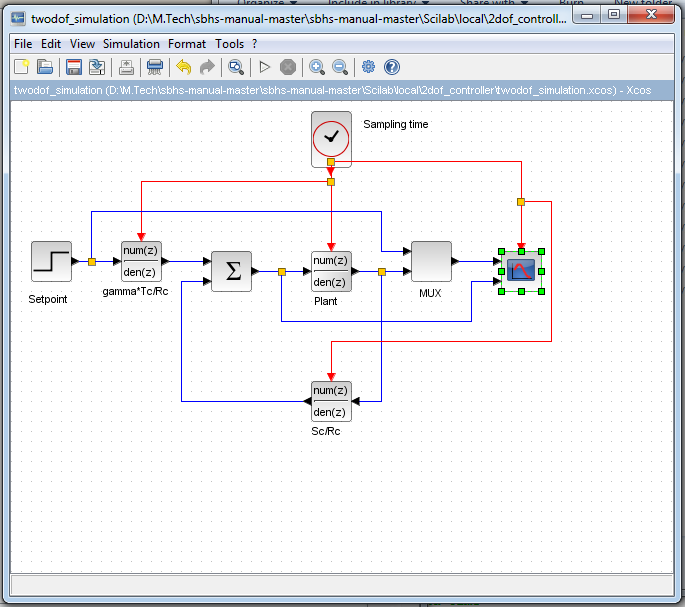
\includegraphics[width=0.8\linewidth]{2-DOF_manual/2dof-sim-xcos}
\caption{Xcos diagram for simulating 2-DOF controller}
\label{2dof-sim-xcos}
\end{figure}

\begin{figure}
\centering
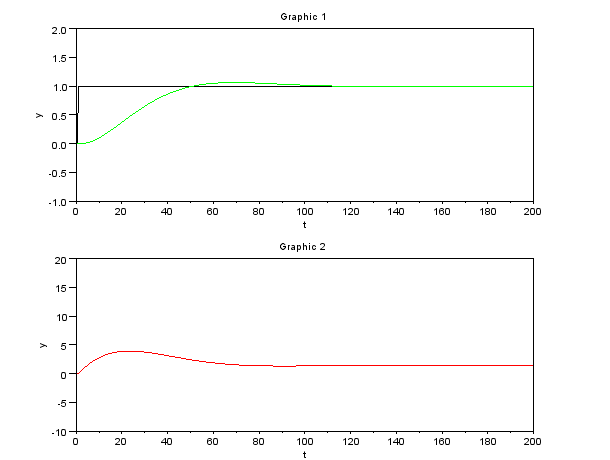
\includegraphics[width=0.8\linewidth]{2-DOF_manual/2dof-sim-result}
\caption{Simulation results after executing  {\tt twodof\_simulation.xcos}}
\label{2dof-sim-res}
\end{figure}
\begin{figure}
\centering
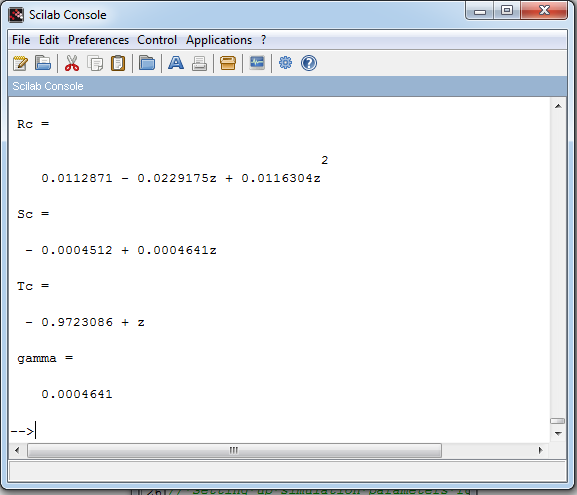
\includegraphics[width=0.8\linewidth]{2-DOF_manual/sci-console}
\caption{Scilab output for \ttfamily twodof\_para.sce}
\label{2dof-para-out}
\end{figure}

\begin{figure}
\centering
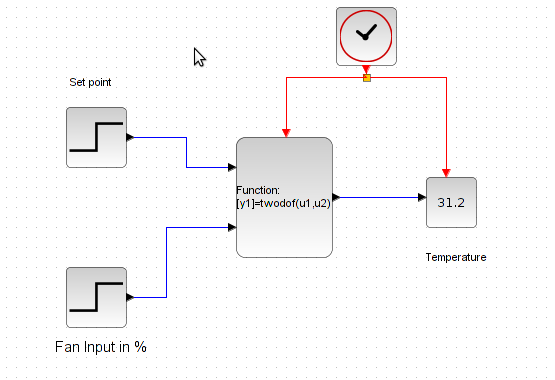
\includegraphics[width=\linewidth]{2-DOF_manual/2dof-xcos}
\caption{Xcos diagram for 2-DOF controller}
\label{2dof-xcos}
\end{figure}
The performance of the controller is shown in figure \ref{rt_127}. 
\begin{figure}
\centering
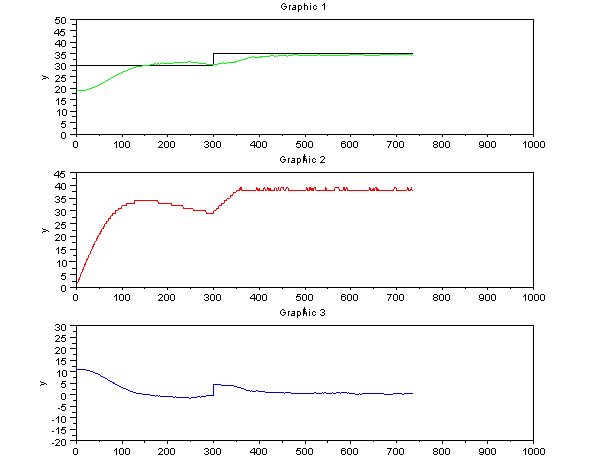
\includegraphics[width=\linewidth]{2-DOF_manual/2dof_resp.png}
\caption{Implementation of 2-DOF controller}
\label{rt_127}
\end{figure}
It is seen that the output (temperature) tracks the setpoint irrespective of the step changes in the fan speed.
We see that the overshoot turns out to be 6\% and rise time turns out to be 60 seconds, which is acceptable.



\section{Scilab Code for Local Experiment} \label{2dof-local}
\begin{code}
\ccaption{twodof\_para.sce}{\ttfamily twodof\_para.sce}
\lstinputlisting{Scilab/local/2dof_controller/twodof_para.sce}
\end{code}
\begin{code}
  \ccaption{twodof.sci }{\ttfamily twodof.sci}
\lstinputlisting{Scilab/local/2dof_controller/twodof.sci}
\end{code}
\begin{code}
  \ccaption{start.sce}{\ttfamily start.sce}
\lstinputlisting{Scilab/local/2dof_controller/start.sce}
\end{code}
\begin{code}
  \ccaption{cindep.sci}{\ttfamily cindep.sci}
\lstinputlisting{Scilab/local/2dof_controller/dc/scilab/cindep.sci}
\end{code}
\begin{code}
  \ccaption{clcoef.sci}{\ttfamily clcoef.sci}
\lstinputlisting{Scilab/local/2dof_controller/dc/scilab/clcoef.sci}
\end{code}
\begin{code}
  \ccaption{colsplit.sci}{\ttfamily colsplit.sci}
\lstinputlisting{Scilab/local/2dof_controller/dc/scilab/colsplit.sci}
\end{code}
\begin{code}
  \ccaption{cosfil\_ip.sci}{\ttfamily cosfil\_ip.sci}
\lstinputlisting{Scilab/local/2dof_controller/dc/scilab/cosfil_ip.sci}
\end{code}
\begin{code}
  \ccaption{indep.sci}{\ttfamily indep.sci}
\lstinputlisting{Scilab/local/2dof_controller/dc/scilab/indep.sci}
\end{code}
\begin{code}
  \ccaption{left\_prm.sci}{\ttfamily left\_prm.sci}
\lstinputlisting{Scilab/local/2dof_controller/dc/scilab/left_prm.sci}
\end{code}
\begin{code}
  \ccaption{makezero.sci}{\ttfamily makezero.sci}
\lstinputlisting{Scilab/local/2dof_controller/dc/scilab/makezero.sci}
\end{code}
\begin{code}
  \ccaption{move\_sci.sci}{\ttfamily move\_sci.sci}
\lstinputlisting{Scilab/local/2dof_controller/dc/scilab/move_sci.sci}
\end{code}
\begin{code}
  \ccaption{polsize.sci}{\ttfamily polisize.sci}
\lstinputlisting{Scilab/local/2dof_controller/dc/scilab/polsize.sci}
\end{code}
\begin{code}
  \ccaption{polyno.sci}{\ttfamily polyno.sci}
\lstinputlisting{Scilab/local/2dof_controller//dc/scilab/polyno.sci}
\end{code}
\begin{code}
  \ccaption{rowjoin.sci}{\ttfamily rowjoin.sci}
\lstinputlisting{Scilab/local/2dof_controller/dc/scilab/rowjoin.sci}
\end{code}
\begin{code}
  \ccaption{seshft.sci}{\ttfamily seshft.sci}
\lstinputlisting{Scilab/local/2dof_controller/dc/scilab/seshft.sci}
\end{code}
\begin{code}
  \ccaption{t1calc.sci}{\ttfamily t1calc.sci}
\lstinputlisting{Scilab/local/2dof_controller/dc/scilab/t1calc.sci}
\end{code}


\section{Scilab Code for Virtual Experiment}\label{2dofcode}
\begin{code}
\ccaption{twodof\_para.sce}{\ttfamily twodof\_para.sce}
\lstinputlisting{Scilab/virtual/2dof_controller/twodof_para.sce}
\end{code}
\begin{code}
  \ccaption{twodof.sce }{\ttfamily twodof.sce}
\lstinputlisting{Scilab/virtual/2dof_controller/twodof.sce}
\end{code}
\begin{code}
  \ccaption{twodof.sci }{\ttfamily twodof.sci}
\lstinputlisting{Scilab/virtual/2dof_controller/twodof.sci}
\end{code}
% \begin{code}
%  \ccaption{comm.sci}{\ttfamily comm.sci}
% \lstinputlisting{Scilab/virtual/2dof_controller/comm.sci}
% \end{code}
% \begin{code}
%  \ccaption{init.sci}{\ttfamily init.sci}
% \lstinputlisting{Scilab/virtual/2dof_controller/init.sci}
% \end{code}

\section{Scilab Codes Common for both Local and Virtual Experiments}
\begin{code}
  \ccaption{myc2d.sci}{\ttfamily myc2d.sci}
\lstinputlisting{Scilab/virtual/2dof_controller/dc/scilab/myc2d.sci}
\end{code}
\begin{code}
  \ccaption{desired.sci}{\ttfamily desired.sci}
\lstinputlisting{Scilab/virtual/2dof_controller/dc/scilab/desired.sci}
\end{code}
\begin{code}
 \ccaption{polmul.sci}{\ttfamily polmul.sci}
\lstinputlisting{Scilab/virtual/2dof_controller/dc/scilab/polmul.sci}
\end{code}
\begin{code}
  \ccaption{polsplit3.sci}{\ttfamily polsplit3.sci}
\lstinputlisting{Scilab/virtual/2dof_controller/dc/scilab/polsplit3.sci}
\end{code}
\begin{code}
 \ccaption{pp\_im.sci}{\ttfamily pp\_im.sci}
\lstinputlisting{Scilab/virtual/2dof_controller/dc/scilab/pp_im.sci}
\end{code}
\begin{code}
 \ccaption{xdync.sci}{\ttfamily xdync.sci}
\lstinputlisting{Scilab/virtual/2dof_controller/dc/scilab/xdync.sci}
\end{code}
\begin{code}
 \ccaption{zpowk.sci}{\ttfamily zpowk.sci}
\lstinputlisting{Scilab/virtual/2dof_controller/dc/scilab/zpowk.sci}
\end{code}
% \begin{code}
%  \ccaption{plotting.sci}{\ttfamily plotting.sci}
% \lstinputlisting{Scilab/virtual/2dof_controller/plotting.sci}
% \end{code}

%\bibliography{2-DOF}

